

A fim de utilizar o método de agrupamento hierárquico para agrupar as estrelas, podemos descobrir o número de agrupamentos ideal para análise de dados via \verb|AgglomerativeClustering|, de modo que num \textit{range} de 2 a 11 \textit{clusters}, podemos visualizar qual é este valor ideal de \textit{clusters}.
\begin{longlisting}
    \begin{minted}{py}
        from sklearn.cluster import AgglomerativeClustering
        from sklearn.metrics import silhouette_score, silhouette_samples
        
        silHier = []
        for n in range(2, 11):
            hier = AgglomerativeClustering(n_clusters=n, linkage='ward')
            labels = hier.fit_predict(scaledNumdS)
            silHier.append(silhouette_score(scaledNumdS, labels))
        
        plt.plot(range(2,11), silHier, marker='o')
        plt.xlabel('Número de Clusters')
        plt.ylabel('Fator de Silhoueta')
        plt.show()
    \end{minted}
\end{longlisting}
\begin{figure}[H]
    \centering
    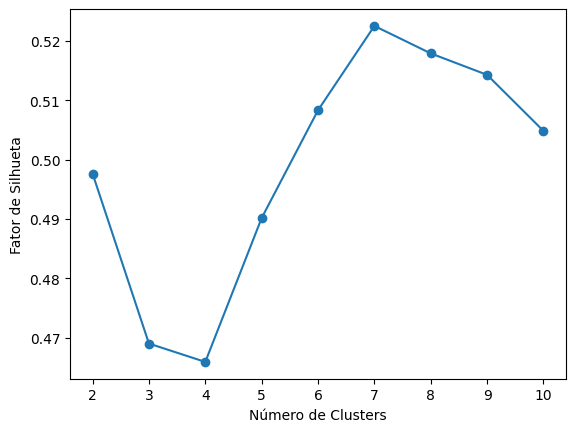
\includegraphics[width=0.5\linewidth]{figures/HierClustSilhouette.png}
\end{figure}
cujo número ideal de \textit{clusters} vai ser definido pelo maior fator de silhueta observado no gráfico, o que podemos gravar no comando
\begin{longlisting}
    \begin{minted}{py}
        bestNumberClustersHier = list(range(2,11))[np.argmax(silHier)]
    \end{minted}
\end{longlisting}
que, para este caso, guardará o valor \verb|bestNumberClusterHier = 7|. Com isso podemos agrupar as estrelas em 7 \textit{clusters}, de tal forma que os gráficos relacionando as características principais das estrelas são facilmente construídos.
\begin{longlisting}
    \begin{minted}{py}
        hierarchical = AgglomerativeClustering(n_clusters=bestNumberClustersHier, linkage='ward').fit(scaledNumdS)
        categoriasHier = hierarchical.labels_

        plt.figure(figsize=(15,10))
        for i, (xVar, yVar) in enumerate([('Temperature', 'L'), ('R','A_M'), ('Temperature','R'), ('L','A_M'), ('Temperature', 'A_M'), ('R','L')], 1):
            plt.subplot(2,3,i)
            plt.scatter(scaledNumdS[xVar], scaledNumdS[yVar], c=categoriasHier, cmap='inferno')
            plt.xlabel(xVar)
            plt.ylabel(yVar)
    \end{minted}
\end{longlisting}
\begin{figure}[H]
    \centering
    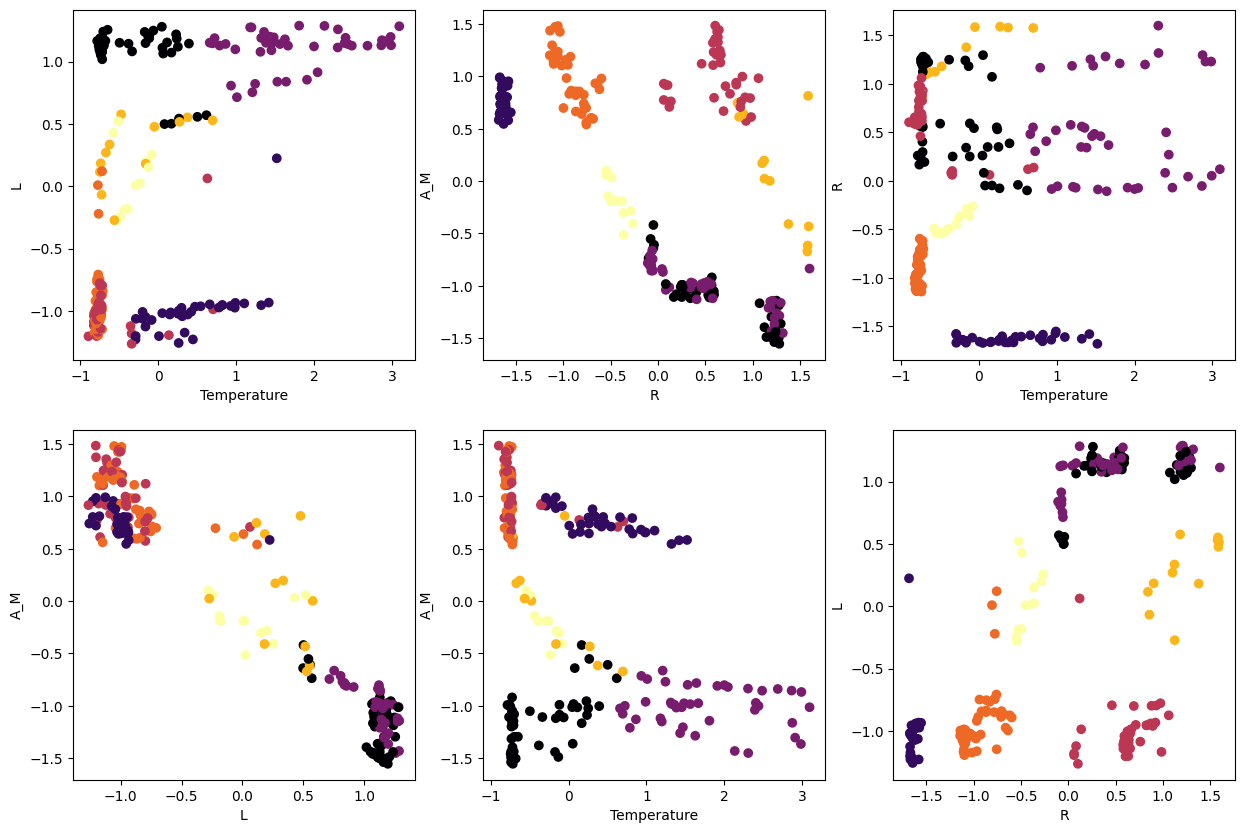
\includegraphics[width=\linewidth]{figures/Hierarchical.png}
\end{figure}

% O método de agrupamento hierárquico mostra uma clusterização interessante ao olharmos principalmente para os gráficos de \verb|A_M| $\times$ \verb|R|, \verb|A_M| $\times$ \verb|Temperature| e \verb|L| $\times$ \verb|R|, pois mesmo que a visualização não seja tão clara, conseguimos ver alguns \textit{clusters} bem formados e separados
